%!TEX root=../thesis.tex
\chapter{Sistemas Lineales}

Nos concentramos, en este capítulo en sistemas planos $\dot{x} = f(x)$ donde la función $f: \R^2 \to \R^2$ es un mapeo lineal. Es decir, el sistema tiene la forma:

\begin{equation} \label{eq:sistemalineal}
	\begin{array}{l}
		\dot{x_1} = a_{11}x_1 + a_{12}x_2 \\
		\dot{x_2} = a_{21}x_1 + a_{22}x_2,
	\end{array}
\end{equation}

donde cada $a_{ij} \in \R$.

Si hacemos

$$ A = \left(
\begin{array}{ll}
	a_{11} & a_{12} \\
	a_{21} & a_{22}
\end{array}
\right),
$$

podemos reescribir el sistema \ref{eq:sistemalineal} en la forma vectorial equivalente

\begin{equation} \label{eq:sistemalinealv}
	\dot{x} = f(x) = Ax.
\end{equation}

Podemos anticipar desde ya que hay un punto crítico del sistema en $\bar{x} = 0$.

\section{Propiedades de las soluciones}

A continuación hacemos un repaso de algunos resultados importantes acerca de las soluciones de sistemas lineales planos autónomos. Las pruebas de los resultados se pueden encontrar en cualquier texto elemental de ecuaciones diferenciales, como podrían ser \cite{zillcull} o \cite{boycediprima}.

\theorem{Todo solución $x$ de un sistema lineal plano tiene la forma $$ x = c_1u+ c_2v, $$ donde $u, v$ son soluciones linealmente independientes de \ref{eq:sistemalinealv} y $c_1, c_2$ son constantes.}

En vista del teorema anterior, el problema se reduce a encontrar dos soluciones $u, v$ que sean linealmente independientes. Tal conjunto de soluciones se conoce como \emph{conjunto fundamental de soluciones} y a $x = c_1u + c_2v$ se le conoce como \textit{solución general}.

Las constantes $c_1$ y $c_2$ quedan determinadas una vez se especifica la condición inicial $x(0) = x^0$.

\begin{lemma}[Criterio para la independencia lineal de soluciones]
Dos soluciones $u$ y $v$ del sistema \ref{eq:sistemalinealv} definidas sobre un intervalo $I$ son linealmente independientes si y sólo si el determinante \emph{wronskiano}

$$ W(u,v)(t) = \left|
	\begin{array}{ll}
		u_1(t) & v_1(t) \\
		u_2(t) & v_2(t)
	\end{array}
\right|$$

es no nulo para toda $t \in I$.
\end{lemma}

\begin{example}
Consideremos el sistema plano

$$
	\begin{array}{l}
		\dot{x_1} = x_1 + 3x_2 \\
		\dot{x_2} = 5x_1 + 3x_2
	\end{array},
$$

que tiene forma vectorial

$$ \dot{x} = \left(
	\begin{array}{ll}
		1 & 3 \\ 5 & 3
	\end{array}
\right) x.$$

Es fácil verificar que las funciones $u(t) = (e^{-2t}, -e^{-2t})$ y $v(t) = (3e^{6t}, 5e^{6t})$ son soluciones del sistema.

Más aún, estas soluciones son linealmente independientes y forman un conjunto fundamental de soluciones pues

$$
	W(u,v)(t) =
\left|
	\begin{array}{ll}
		e^{-2t} & 3e^{6t} \\
		-e^{-2t} & 5e^{6t}
	\end{array}
\right| = 5e^{4t} + 3e^{4t} = 8e^{4t} \neq 0,
$$

para todo $t \in \R$.

Esto significa que toda solución del sistema tiene la forma

$$ x(t) = \left( \begin{array}{l} x_1(t) \\ x_2(t) \end{array} \right)
= c_1 \left( \begin{array}{l} e^{-2t} \\ -e^{-2t} \end{array} \right) + c_2 \left( \begin{array}{l} 3e^{6t} \\ 5e^{6t} \end{array} \right).$$
\end{example}

Por analogía a la teoría de ecuaciones diferenciales lineales de primer orden (ver, por ejemplo, \cite{zillcull,boycediprima}), buscamos soluciones del sistema \ref{eq:sistemalinealv} que tengan la forma
\begin{equation} \label{eq:solexponencial}
x(t) = (k_1e^{\lambda t}, k_2e^{\lambda t}).
\end{equation}

Supongamos que $x$ es una solución de la forma \ref{eq:solexponencial}. Entonces

$$ \dot{x} = (k_1 \lambda e^{\lambda t}, k_2 \lambda e^{\lambda t}). $$

Si reemplazamos $x$ y $\dot{x}$ en la ecuación $\dot{x} = f(x) = Ax$ y hacemos $K = (k_1, k_2)$ obtenemos

$$
	K \lambda e^{\lambda t} = A (Ke^{\lambda t}).
$$

Como $e^{\lambda t} \neq 0$ podemos dividir ambos lados de la ecuación anterior por $e^{\lambda t}$ y reordenando se obtiene

$$ AK = \lambda K$$

o equivalentemente

\begin{equation} \label{eq:ecvalorpropio}
	(A - \lambda I) K = 0.
\end{equation}

Lo anterior significa que si $x = x(t)$ es una solución de la forma propuesta, entonces $\lambda$ y $K$ deben satisfacer \ref{eq:ecvalorpropio}. Es decir, $\lambda$ debe ser un valor propio de $A$ y $K$ un vector propio asociado a este valor propio $\lambda$.

En estas condiciones, $$ x = K e^{\lambda t}$$ es siempre solución de $\dot{x} = Ax$.

El resto de esta sección está dedicado a la obtención de dos soluciones que sean linealmente independientes $u$ y $v$ de manera que podamos escribir siempre la solución general de la forma antes descrita en términos de estas dos soluciones.

En virtud de lo anterior es lógico que las soluciones dependan de la forma de los valores propios de $A$: como $\det(A - \lambda I) = 0$ es una ecuación algebraica de segundo grado, estos pueden ser reales y distintos, reales repetidos o complejos conjugados.

\subsection{Ecuación Característica}

Para hallar los valores propios $\lambda$ de la matriz $A$ 2x2 del sistema \ref{eq:sistemalinealv} computamos las raíces de la ecuación característica $\det(A - \lambda I) = 0$.

Notamos que
\begin{eqnarray*}
	\det(A - \lambda I) & = &  \left| \begin{array}{ll} a_{11} - \lambda & a_{12} \\ a_{21} & a_{22} - \lambda \end{array} \right| \\ 
	& = & (a_{11} - \lambda)(a_{22} - \lambda) - a_{12}a_{21} \\
	& = & \lambda^2 - (a_{11} + a_{22})\lambda + (a_{11}a_{22} - a_{12}a_{21}).
\end{eqnarray*}

Si escribimos $\Delta = \det(A) = a_{11}a_{22} - a_{12}a_{21}$ y $\tau = a_{11} + a_{22}$, la traza de $A$, entonces la ecuación característica es:

\begin{equation} \label{eq:eccaracteristica}
	\lambda^2 - \tau \lambda + \Delta = 0.
\end{equation}

Por lo tanto los valores propios de $A$ son $\lambda_{1,2} = (\tau \pm \sqrt{\tau^2 - 4\Delta}) / 2 $ que pueden ser reales distintos, reales repetidos y complejos conjugados según $\tau^2 - 4\Delta$ sea positivo, cero o negativo.

\subsection{Solución General} \label{subsec:soluciongeneral}

Enunciamos, sin prueba, un teorema acerca de la solución general del sistema para cada uno de estos casos.

\begin{theorem}[Solución para valores propios reales distintos]Si $\tau^2 - 4\Delta > 0$ entonces la ecuación característica \ref{eq:eccaracteristica} tiene dos raíces reales $\lambda_1$ y $\lambda_2$ distintas y la solución general del sistema lineal plano $\dot{x} = Ax$ está dada por

\begin{equation} \label{eq:solvlrspropiosdistintos}
x = x(t) = c_1(K_1 e^{\lambda_1 t}) + c_2(K_2 e^{\lambda_2 t}),
\end{equation}

donde $K_1$ es un vector propio asociado al valor propio $\lambda_1$ y $K_2$ uno asociado al valor propio $\lambda_2$.
\end{theorem}

\begin{theorem}[Solución para valores propios reales repetidos]Si $\tau^2 - 4\Delta = 0$ entonces la ecuación característica \ref{eq:eccaracteristica} tiene una raíz real $\lambda_1$ de multiplicidad dos.

\begin{itemize}

\item Si existen dos vectores propios linealmente independientes $K_1, K_2$ asociados a $\lambda_1$ entonces la solución general del sistema lineal plano $\dot{x} = Ax$ está dada por

\begin{equation} \label{eq:solvlrspropiosrepetidos1}
x = x(t) = c_1(K_1 e^{\lambda_1 t}) + c_2(K_2 e^{\lambda_1 t}).
\end{equation}

\item Si sólo se tiene un vector propio linealmente independiente $K_1$ entonces la solución general del sistema lineal plano $\dot{x} = Ax$ tiene la forma

\begin{equation} \label{eq:solvlrspropiosrepetidos2}
x = x(t) = c_1(K_1 e^{\lambda_1 t}) + c_2(K_1 t e^{\lambda_1 t} + Pe^{\lambda_1 t}),
\end{equation}

donde $P$ es un vector tal que $(A-\lambda_1I)P=K_1$.
\end{itemize}

\end{theorem}


\begin{theorem}[Solución para valores propios complejos conjugados]Si $\tau^2 - 4\Delta < 0$ entonces la ecuación característica \ref{eq:eccaracteristica} tiene dos raíces complejas conjugadas $\lambda_{1,2} = a \pm i b$ y la solución general del sistema lineal plano $\dot{x} = Ax$ está dada por

\begin{equation} \label{eq:solvlrspropioscomplejos}
x = x(t) = c_1 e^{a t}(B_1 \cos(bt) - B_2 \sin(bt)) + c_2 e^{a t}(B_2 \cos(bt) + B_1 \sin(bt)),
\end{equation}

donde $K_1 = B_1 + iB_2$ es un vector propio asociado al valor propio $\lambda_1$.
\end{theorem}

\section{Clasificación y estabilidad de puntos críticos ($\Delta \neq 0$)} \label{sec:estabilidadlineal}

Si $A$ es no singular ($\det(A) = \Delta \neq 0$), el único punto crítico del sistema lineal plano $\dot{x} = f(x) = Ax$ es $\bar{x} = 0$.

El comportamiento cualitativo de las soluciones que no son de equilibrio, en un sistema lineal, es muy similar y nos permite establecer una clasificación para el punto crítico $\bar{x} = 0$.

Hemos visto ya en ejemplos anteriores que algunas soluciones se alejan o acercan a los puntos críticos, otras se enrollan alrededor del punto crítico, etc. A continuación justificaremos cada uno de estos posibles casos según sean los valores propios de $A$ (como se vio en la sección anterior).

\subsection{Valores propios reales distintos y negativos (nodo estable)}
Consideramos el caso $\tau^2 - 4\Delta > 0$ y $\lambda_1, \lambda_2$ son valores propios de $A$ tales que $\lambda_1 < 0, \lambda_2 < 0$.

En este caso, toda solución es de la forma \ref{eq:solvlrspropiosdistintos}:

$$ x = c_1(K_1 e^{\lambda_1 t}) + c_2(K_2 e^{\lambda_2 t}). $$

Podemos reescribir la solución como

$$ x = e^{\lambda_1 t} [ c_1 K_1 + c_2K_2 e^{(\lambda_2 - \lambda_1)t} ].$$

Supongamos sin pérdida de generalidad que $\lambda_2 < \lambda_1 < 0$, entonces de acuerdo a la ecuación anterior $x(t) \to 0$ cuando $t \to \infty$.
A largo plazo, $x(t) \approx c_1K_1e^{\lambda_1 t}$ y por lo tanto si $c_1 \neq 0$ entonces $x \to 0$ a lo largo de la recta determinada por el vector propio $K_1$.
Si en cambio, $c_1 = 0$ entonces $x(t) = c_2 K_2 e^{\lambda_2 t}$ y $x \to 0$ desde una de las direcciones determinadas por el vector propio $K_2$.

En particular si el punto inicial $x^0$ está en alguna de las rectas determinadas por $K_1$ o $K_2$ la solución tiende a 0 a través de la recta.

En cualquier caso, $x \to 0$ y decimos que el punto crítico $\bar{x} = 0$ es un \emph{nodo (estable)} o \emph{sumidero nodal}.

\subsection{Valores propios reales distintos y positivos (nodo inestable)}

Como antes, $\tau^2 - 4\Delta > 0$ pero ahora $\lambda_1 > 0$ y $\lambda_2 > 0$.
Toda solución solución puede escribirse también como

$$ x = e^{\lambda_1 t} [ c_1 K_1 + c_2K_2 e^{(\lambda_2 - \lambda_1)t} ].$$

Supondremos, de nuevo, que $\lambda_1 > \lambda_2$. Entonces a largo plazo $|x(t)| \approx |c_1 K_1 e^{\lambda_1 t}| \to \infty$ cuando $t \to \infty$.

El patrón de las trayectorias es idéntico al caso anterior pero estas se alejan del punto crítico $\bar{x} = 0$ en lugar de acercarse. En este caso el punto crítico $\bar{x} = 0$ se llama \emph{nodo (inestable)} o \emph{sumidero nodal}.

\begin{figure}[!ht] \centering
    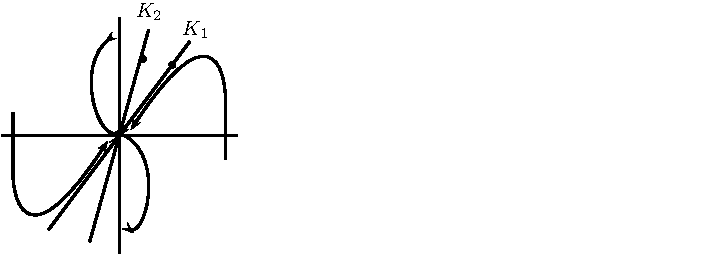
\includegraphics[scale=1.0]{figures/nodoestable.pdf}\\(a)\\
    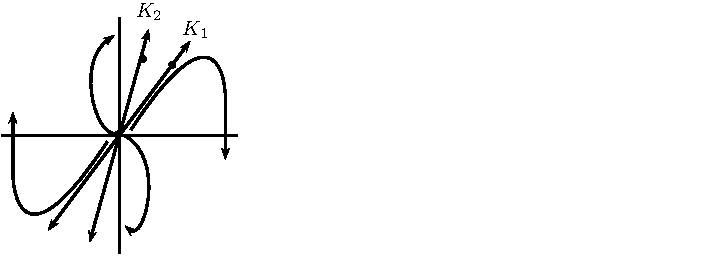
\includegraphics[scale=1.0]{figures/nodoinestable.pdf}\\(b)\\
    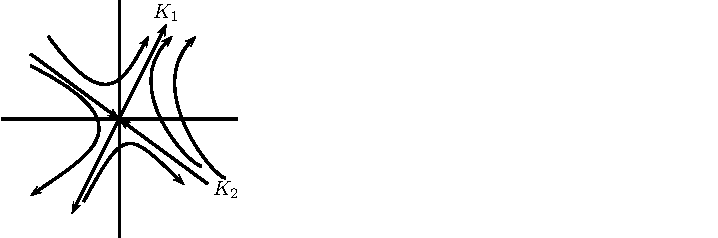
\includegraphics[scale=1.0]{figures/puntodesilla.pdf}\\(c)\\
    \caption{(a) Nodo estable, (b) Nodo inestable, (c) Punto de silla.}
	\label{fig:nodos}
\end{figure}

\subsection{Valores propios reales distintos y de signo opuesto (punto de silla)}

De nuevo la solución es de la forma

$$ x = c_1(K_1 e^{\lambda_1 t}) + c_2(K_2 e^{\lambda_2 t}). $$

Suponemos que $\lambda_2 < \lambda_1$.

Si $c_1 = 0$ (por ejemplo, cuando $x^0$ está sobre la recta determinada por $K_2$) entonces como $\lambda_2 < 0$, $x \to 0$ a lo largo de esta recta.
Si $c_2 = 0$ (por ejemplo, cuando $x^0$ está sobre la recta determinada por $K_1$) entonces dado que $\lambda_1 >0$, $||x|| \to \infty$ a lo largo de la recta determinada por $K_1$.

Las soluciones que parten de otros puntos iniciales, para las cuales $c_1 \neq 0$ y $c_2 \neq 0$ el término dominante en la solución es $e^{\lambda_1 t}$ y como $\lambda_1 > 0$ entonces las soluciones se hacen no acotadas a medida que aumenta $t$ de manera asintótica a la recta determinada por $K_1$.

Resumiendo, las soluciones que no comienzan en ninguna de las rectas determinadas por $K_1$ o $K_2$ son tales que $||x|| \to \infty$ y lo hacen de manera asintótica a la recta determinada por $K_1$. De otro lado, las únicas soluciones que tienden al punto de equilibrio $\bar{x} = 0$ son aquellas que comienzan sobre la recta determinada por $K_2$ y lo a lo largo de dicha recta.

En este caso, el punto crítico se llama \emph{punto de silla} y es, evidentemente, un equilibrio inestable.

\subsection{Valor propio real repetido (nodo degenerado)}

En este caso $\tau^2 - 4\Delta = 0$ y hay un único valor propio real de multiplicidad dos: $\lambda_{1,2} = \lambda$.

\subsubsection{Dos vectores propios linealmente independientes (nodo propio degenerado)}

Si se pueden conseguir dos vectores propios $K_1$ y $K_2$ linealmente independientes asociados al valor propio $\lambda$ entonces toda solución es de la forma \ref{eq:solvlrspropiosrepetidos1}, que puede reescribirse como
$$ x = (c_1K_1 + c_2K_2)e^{\lambda t}.$$

En este caso el punto crítico $\bar{x} = 0$ se dice \emph{nodo propio}, \emph{nodo degenerado} o \emph{punto estrella} y es estable o inestable según $\lambda < 0$ o $\lambda > 0$ respectivamente.

\begin{figure}[!ht] \centering
    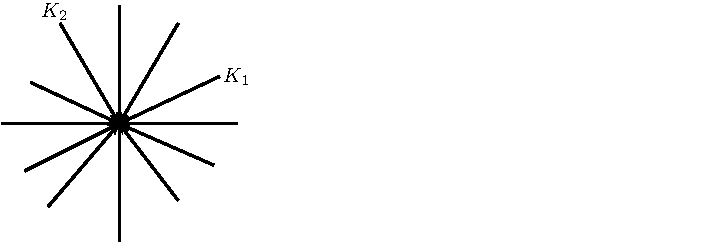
\includegraphics[scale=1.0]{figures/nodopropio.pdf}
    \caption{Nodo propio degenerado.}
	\label{fig:nodopropio}
\end{figure}

\subsubsection{Un solo vector linealmente independiente (nodo impropio degenerado)}

En este caso apenas es posible conseguir un vector propio $K_1$ linealmente independiente asociado al valor propio $\lambda$. Las soluciones, según la fórmula \ref{eq:solvlrspropiosrepetidos2}, son de la forma:
$$ x =c_1(K_1 e^{\lambda t}) + c_2(K_1 t e^{\lambda t} + Pe^{\lambda t}). $$

El comportamiento de todas las soluciones $x = x(t)$ es similar: la recta determinada por $K_1$ es una asíntota y $||x|| \to 0$ si $\lambda < 0$ o $||x|| \to \infty$ si $\lambda > 0$.

Si $\lambda < 0$ entonces el punto crítico $\bar{x} = 0$ se llama \emph{nodo impropio estable} o simplemente \emph{nodo degenerado estable} y si $\lambda > 0$ el punto crítico $\bar{x} = 0$ se llama \emph{nodo impropio inestable} o \emph{nodo generado inestable}.

\begin{figure}[!ht] \centering
    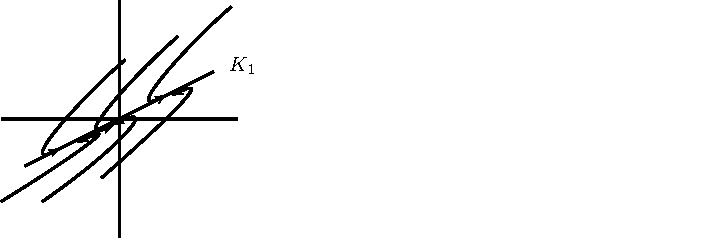
\includegraphics[scale=1.0]{figures/nodoimpropio.pdf}
    \caption{Nodo impropio degenerado.}
	\label{fig:nodoimpropio}
\end{figure}

\subsection{Valores propios complejos conjugados (centro, punto de espiral)} \label{subsec:centrooespiral}

Finalmente, estamos en el caso en el que $\tau^2 - 4\Delta < 0$ y los valores propios de $A$ son complejos conjugados: $\lambda_{1,2} = a \pm ib$.

Si $K_1 = B_1 + iB_2$ es un vector propio asociado al valor propio $\lambda_1 = a + ib$ entonces, por la fórmula \ref{eq:solvlrspropioscomplejos} la solución es de la forma

$$ x = c_1 e^{a t}(B_1 \cos(bt) - B_2 \sin(bt)) + c_2 e^{a t}(B_2 \cos(bt) + B_1 \sin(bt)).$$

\subsubsection{Valor propio imaginario puro}
Cuando $\tau = 0$, $\lambda_1$ es un imaginario puro y la solución se puede escribir como

$$ x = C_1 \cos(bt) + C_2 \sin(bt), $$

donde $C_1$ y $C_2$ son vectores constantes. Esto implica que todas las soluciones son periódicas con período $2\pi / b$ y es fácil ver que corresponden a elipses centradas en el origen.

En este caso el punto crítico $\bar{x} = 0$ se llama \emph{centro} y la orientación de todas las órbitas es la misma.

\subsubsection{Valor propio con parte real no nula}

Si $\tau \neq 0$ entonces los valores propios tienen parte real $a \neq 0$ y las órbitas del sistema son espirales que se alejan o acercan todas al punto crítico $\bar{x} = 0$ debido al término $e^{a t}$ que aparece en la solución.

El punto crítico se llama un \emph{punto espiral} y es estable cuando $\lambda < 0$ e inestable cuando $\lambda > 0$.

Cuando el punto espiral es estable se le llama también \emph{sumidero espiral} y cuando es inestable \emph{fuente espiral}.

\begin{figure}[!ht] \centering
    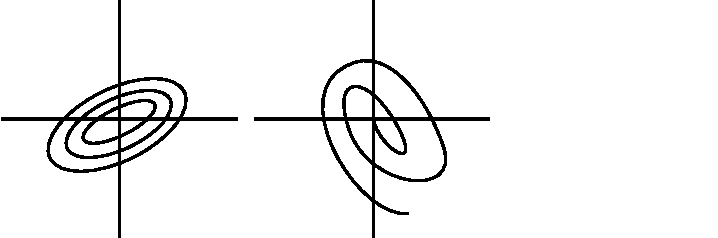
\includegraphics[scale=1.0]{figures/centroyespiral.pdf}  
    \caption{Centro y punto de espiral.}
	\label{fig:centroyespiral}
\end{figure}

\section{Clasificación y estabilidad de puntos críticos ($\Delta = 0$)}

Cuando el sistema plano es $\dot{x} = f(x) = Ax$ con $A$ una matriz singular (i.e. $\det(A) = \Delta = 0$) entonces es un resultado elemental del álgebra lineal que hay una infinidad de puntos críticos (soluciones a $Ax = 0$) además del origen $x = 0$.

Las soluciones en la sección \ref{subsec:soluciongeneral} siguen siendo válidas en este caso, aunque se advierte ya de la ecuación característica \ref{eq:eccaracteristica} que los valores propios son $\lambda_1 = 0$ y $\lambda_2 \in \R$.

Consideramos a continuación varios casos.

\subsection{A es la matriz cero ($A = 0$)}
En este caso todo punto $x \in \R^2$ es un punto crítico, así que toda trayectoria en el plano de fase es trivial.

\begin{figure}[!ht] \centering
    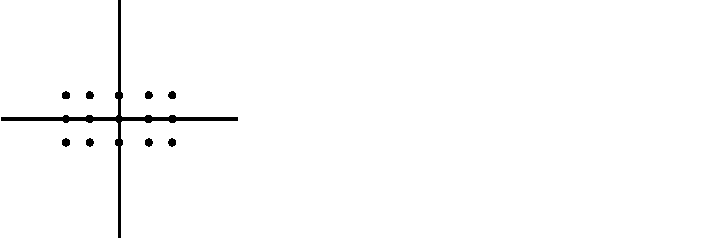
\includegraphics[scale=1.0]{figures/amatriz0.pdf}  
\end{figure}


\subsection{$\lambda_1 = 0, \lambda_2 < 0$}
Es posible demostrar que en este caso el sistema es topológicamente equivalente (ver \cite[p.~239]{dynandbif}) a uno con matriz de coeficientes

$$ A = \left( \begin{array}{ll} -1 & 0 \\ 0 & 0 \end{array} \right).$$

Por lo tanto, el diagrama de fase es similar a la figura siguiente, donde todo punto $(0,x_2)$ es de equilibrio.

\begin{figure}[!ht] \centering
    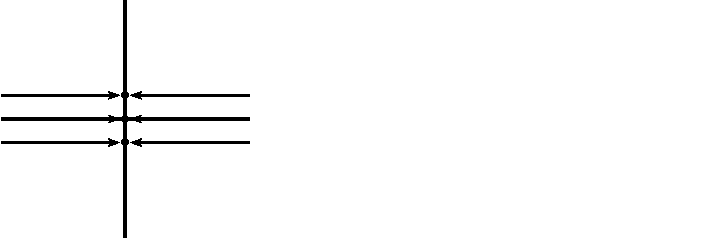
\includegraphics[scale=1.0]{figures/asingular_1.pdf}
\end{figure}

\subsection{$\lambda_1 = 0, \lambda_2 > 0$}
De nuevo, como en \cite[p.~239]{dynandbif}, es posible verificar que este sistema es topológicamente equivalente a uno con matriz de coeficientes

$$ A = \left( \begin{array}{ll} 1 & 0 \\ 0 & 0 \end{array} \right).$$

Por lo tanto, el diagrama de fase es similar a la figura siguiente, donde todo punto $(0,x_2)$ es de equilibrio pero el sentido de las flechas es contrario al del caso anterior.

\begin{figure}[!ht] \centering
    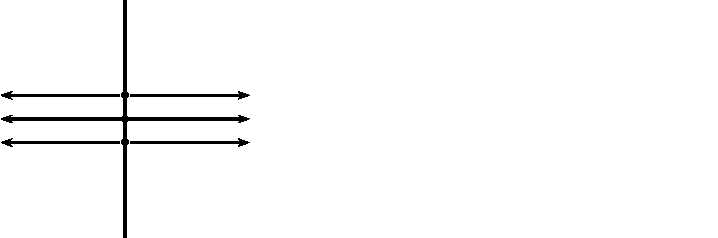
\includegraphics[scale=1.0]{figures/asingular1.pdf}
\end{figure}

\subsection{$\lambda_1 = \lambda_2 = 0$}
En este caso tanto $\Delta$ como $\tau$ son nulos. Esto es, $a_{11}a_{22} - a_{12}a_{21} = 0$ y también $a_{11} + a_{22} = 0$.
Es posible analizar el comportamiento de las soluciones y puntos de equilibrio a partir de estas ecuaciones considerando los distintos casos $a_{11} = 0$ o $a_{11} \neq 0$, etc.

Sin embargo, cualquiera sea el caso el sistema es equivalente (ver \cite[teorema 8.16 p.~239]{dynandbif}) a uno con matriz de coeficientes

$$ A = \left( \begin{array}{ll} 0 & 1 \\ 0 & 0 \end{array} \right),$$

cuyo diagrama de fase aparece es como a continuación.

\begin{figure}[!ht] \centering
    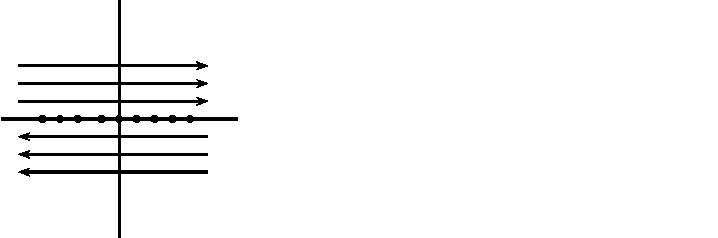
\includegraphics[scale=1.0]{figures/asingularr1.pdf}
\end{figure}

\begin{remark}Aunque no se dijo explícitamente para cada caso, es claro que todos los puntos de equilibrio son \emph{inestables} si $\Delta = 0$.
\end{remark}

\section{Criterio de estabilidad para sistemas lineales}
Resumimos los resultados de las dos secciones previas:

\begin{theorem}[Criterio de estabilidad para sistemas lineales] \label{teo:criterioestabilidadlineales}
Sea $\dot{x} = f(x) = Ax$ un sistema plano lineal y $\bar{x}$ un punto de equilibrio del mismo.

\begin{enumerate}[(a)]
	\item Si $\det(A) \neq 0$ y todos los valores propios de $A$ tienen parte real negativa o son imaginarios puros, $\bar{x} = 0$ es un punto crítico asintóticamente estable (y por tanto estable).
	\item Si $\det(A) = 0$ o hay valores propios de $A$ con parte real positiva, el punto crítico $\bar{x}$ es inestable.
\end{enumerate}

Debido a lo anterior a menudo la clasificación de puntos críticos y estabilidad se realiza según los valores propios de $A$ tengan o no parte real no nula.

\begin{definition}[Matriz hiperbólica] Decimos que $A$ es \emph{hiperbólica} si todos sus valores propios tienen parte real no nula.
\end{definition}

Con esta definición, notamos que la estabilidad de un punto de equilibrio de un sistema lineal con matriz de coeficientes hiperbólica depende exclusivamente del signo de la parte real.

\end{theorem}

